\documentclass[submit]{../harvardml}

\course{CS1810-S25}
\assignment{Homework \#2}
\duedate{February 28, 2025 at 11:59 PM}

\usepackage{../common}
\usepackage[OT1]{fontenc}
\usepackage[colorlinks,citecolor=blue,urlcolor=blue]{hyperref}
\usepackage{graphicx}
\usepackage{subfig}
\usepackage{fullpage}
\usepackage{amsmath}
\usepackage{amssymb}
\usepackage{framed}
\usepackage{color}
\usepackage{soul}
\usepackage{todonotes}
\usepackage{listings}
\usepackage{enumitem}
\usepackage{bm}
\usepackage{bbm}


\newcommand{\B}{\text{B}}
\newcommand{\Beta}{\text{Beta}}

\usepackage[mmddyyyy,hhmmss]{datetime}

\definecolor{verbgray}{gray}{0.9}

\lstnewenvironment{csv}{%
  \lstset{backgroundcolor=\color{verbgray},
  frame=single,
  framerule=0pt,
  basicstyle=\ttfamily,
  columns=fullflexible}}{}
  

%%%%%%%%%%%%%%%%%%%%%%%%%%%%%%%%%%%%%%%%%%%
%% Solution environment
\usepackage{xcolor}
\newenvironment{solution}{
    \vspace{2mm}
    \color{blue}\noindent\textbf{Solution}:
}{}
%%%%%%%%%%%%%%%%%%%%%%%%%%%%%%%%%%%%%%%%%%%


\begin{document}

\begin{center}
  {\Large Classification and Bias-Variance Trade-offs}\\
\end{center}

\subsection*{Introduction}

This homework is about classification, bias-variance trade-offs, and
uncertainty quantification.

The datasets that we will be working with relate to astronomical observations and loan applicants
The first dataset, found at \verb|data/planet-obs.csv|,
contains information on whether a planet was observed (as a binary
variable) at given points in time. This will be used in Problem 1. The
second dataset, available at \verb|data/hr.csv|, details different
loan applicants and their measured debt to income ratio and credit score. You will
work with this data in Problem 3.

As a general note, for classification problems we imagine that we have
the input matrix $\boldX \in \reals^{n \times d}$ (or perhaps they
have been mapped to some basis $\bm{\Phi}$, without loss of
generality) with outputs now ``one-hot encoded."  This means that if
there are~$K$ output classes, rather than representing the output
label $y$ as an integer~${1,2,\ldots,K}$, we represent $\boldy$ as a
``one-hot" vector of length~$K$. A ``one-hot" vector is defined as
having every component equal to 0 except for a single component which
has value equal to 1.  For example, if there are $K = 7$ classes and a
particular data point belongs to class 3, then the target vector for
this data point would be~$\boldy = [0,0,1,0,0,0,0]$.  We will define
$C_1$ to be the one-hot vector for the 1st class, $C_2$ for the 2nd
class, etc.  Thus, in the previous example $\boldy = C_3$. If there
are $K$ total classes, then the set of possible labels is $\{C_1
  \ldots C_K \} = \{C_k\}_{k=1}^K$.  Throughout the assignment we will
assume that each label $\boldy \in \{C_k\}_{k=1}^K$ unless otherwise
specified. The most common exception is the case of binary
classification ($K = 2$), in which case labels are the typical
integers $y \in \{0, 1\}$.

\subsection*{Resources and Submission Instructions}

We encourage you to read CS181 Textbook's Chapter 3 for more
information on linear classification, gradient descent, and
classification in the discriminative setting. Read Chapter 2.8 for
more information on the trade-offs between bias and variance.

In problems 1 and 3, you may use \texttt{numpy} or \texttt{scipy}, but
not \texttt{scipy.optimize} or \texttt{sklearn}. Example code is given
in the provided notebook. \textbf{We highly recommend that you use Google Colab for problems 1 and 3 to avoid numerical stability issues.}

Please type your solutions after the corresponding problems using this
\LaTeX\ template, and start each problem on a new page.

Please submit the \textbf{writeup PDF to the Gradescope assignment
  `HW2'}. Remember to assign pages for each question.  Please submit
your \textbf{\LaTeX\ file and code files to the Gradescope assignment
  `HW2 - Supplemental'}. \textbf{You must include your plots in your
  writeup PDF. } The supplemental files will only be checked in
special cases, e.g. honor code issues, etc.


%%%%%%%%%%%%%%%%%%%%%%%%%%%%%%%%%%%%%%%%%%%%%
% Problem 1
%%%%%%%%%%%%%%%%%%%%%%%%%%%%%%%%%%%%%%%%%%%%%

\begin{problem}[Exploring Bias-Variance and Uncertainty]
In this problem, we will explore the bias and variance of a few
different model classes when it comes to logistic regression and
investigate two sources of predictive uncertainty in a synthetic
(made-up) scenario.

We are using a powerful telescope in the northern hemisphere to gather
measurements of some planet of interest. At certain times however, our
telescope is unable to detect the planet due to its positioning around
its star.  The data in \verb|data/planet-obs.csv| records the
observation time in the ``Time" column and whether the planet was
detected in the ``Observed" column (with the value 1 representing that
it was observed).  These observations were taken over a dark, clear
week, which is representative of the region.  Since telescope time is
expensive, we would like to build a model to help us schedule and find
times when we are likely to detect the planet.

\begin{enumerate}
  \item Split the data into 10 mini-datasets of size $N = 30$ (i.e. dataset 1 consists of the first 30 observations, dataset 2 consists of the next 30, etc. This has already been done for you). Consider the three bases $\boldsymbol\phi_1(t) = [1, t]$, $\boldsymbol\phi_2(t) = [1,
          t, t^2]$, and $\boldsymbol\phi_3(t) = [1, t, t^2, t^3, t^4, t^5]$. For each of these bases, fit a logistic regression model using sigmoid($\boldw^\top \boldsymbol\phi(t)$) to each dataset by using gradient descent to
        minimize the negative log-likelihood.  This means you will be
        running gradient descent 10 times for each basis, once for each
        dataset.

        Use the given starting values of $\boldw$ and a learning rate of $\eta=0.001$, take 1,000 update
        steps for each gradient descent run, and make sure to average the
        gradient over the data points at each step. These parameters,
        while not perfect, will ensure your code runs reasonably quickly.

  \item After consulting with a domain expert, we find that the probability of observing the planet is periodic as the planet revolves around its star---we are more likely to observe the planet when it is in front of its star than when it is behind it. In fact, the expert determines that observation follows the generating process $y \sim \text{Bern}(f(t))$, where $f(t) = 0.4 \times \cos(1.1t + 1) + 0.5$ for $t \in [0, 6]$ and $y \in \{0,1\}$. Note that we, the modelers, do not usually see the true data distribution. Knowledge of the true $f(t)$ is only exposed in this problem to allow for verification of the true bias.

        Use the given code to plot the true process versus your learned models. Include your plots in your solution PDF.

        \textbf{In no more than 5 sentences}, explain how bias and variance reflected in the 3 types of curves on the graphs.  How do the fits of the individual and mean prediction functions change?  Keeping in mind that none of the model classes match the true generating process exactly, discuss the extent to which each of the bases approximates the true process.

\end{enumerate}
\end{problem}

\newpage
\begin{framed}
  \noindent\textbf{Problem 1} (cont.)\\
  \begin{enumerate}
    \setcounter{enumi}{2}

    \item If we were to increase the size of each dataset drawn from $N = 30$ to a larger number, how would the bias and variance change for each basis? Why might this be the case? You may experiment with generating your own data that follows the true process and plotting the results, but this is \textbf{not} necessary. \textbf{Your response should not be longer than 5 sentences}.

    \item Consider the test point $t = 0.1$. Using your models trained on basis $\boldsymbol\phi_3$, report the predicted probability of observation of the \textit{first} model (the model trained on the first 30 data points). How can we interpret this probability as a measure of uncertainty? Then, compute the variance of the classification probability over your 10 models at the same point $t = 0.1$. How does this measurement capture another source of uncertainty, and how does this differ from the uncertainty represented by the classification probability? Repeat this process (reporting the first model's classification probability and the variance over the 10 models) for the point $t = 3.2$.

          Compare the uncertainties and their sources at times $t=0.1$ and $t=3.2$.

    \item We now need to make some decisions about when to request time on
          the telescope.  The justifications of your decisions will be sent to
          your funding agency, which will determine whether you will be
          allocated funds to use the telescope for your project. \textbf{In no more than 10 lines}, answer the following questions.
          \begin{itemize}
            \item To identify the ideal time, which model(s) would you use and why?
            \item What time would you request, and why?
            \item Your funding agency suggests using a different telescope in a
                  humid area near the equator. Can you still use your model to
                  determine when the planet is likely to be visible?  Why? Are there
                  adaptations that may be necessary?
            \item You seek out a team that has used the alternative telescope
                  for observing this planet, and they provide you their observation
                  file \verb|data/planet-obs-alternate.csv|.
                  Compare the observations from your telescope to theirs.  What
                  seems to be happening?  What might be an appropriate model for
                  this? Your funding agency asks you to refit your models on these
                  new data.  Do you think this is a reasonable ask, and if so, how
                  will it help you make better decisions about when to request
                  viewing time?  If not, why do you think the additional modeling
                  will not help? You do \emph{not} need to do any modeling for this
                  question!

          \end{itemize}
          In these questions, we are looking for your reasoning; there may be
          more than one valid answer.

  \end{enumerate}
\end{framed}

\newpage

\begin{solution}
	\begin{itemize}
    \item[2.] We have the following:
    \begin{center}
      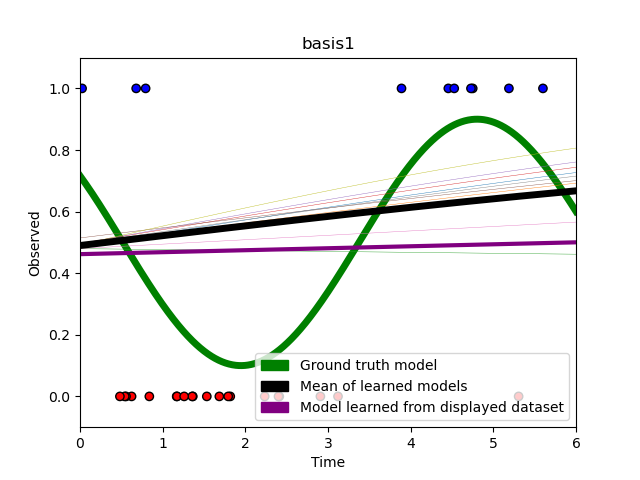
\includegraphics[width=0.5\textwidth]{img_output/basis1.png}
      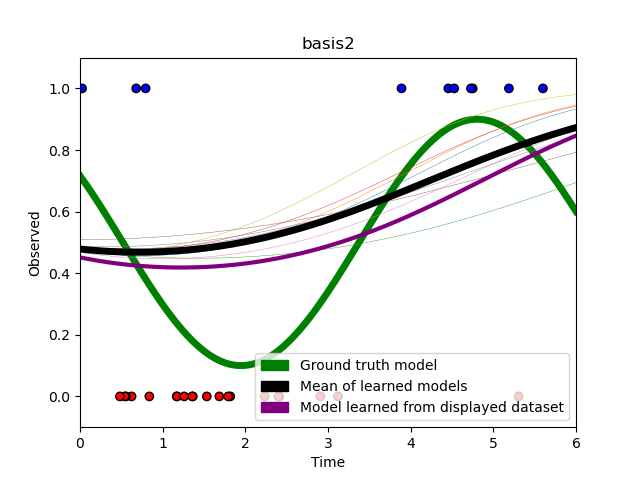
\includegraphics[width=0.5\textwidth]{img_output/basis2.png}
      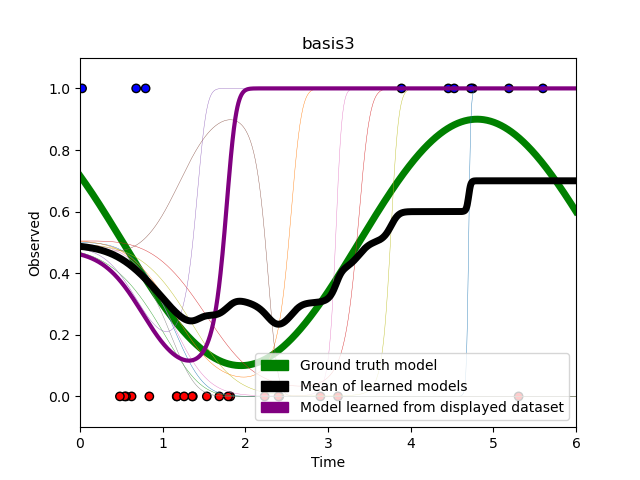
\includegraphics[width=0.5\textwidth]{img_output/basis3.png}
    \end{center}
    Note that as we go from basis1 to basis3, the curves get progressive more crazy while adhering to the curve itself better (bias going down while variance goes up). We can also watch the progression from underfit to overfit by observing the mean of learned models - the mean of the learned models almost has the sinusoidal shape of the true process in basis3, but there are many more fluctuations in the curve. \par
    Basis1 is pretty trash, with wild underfitting, and basis2 is a tiny bit better but also quite bad. 
    \item[3)] We implement this, and we see that the bias plateaus while the variance continues to decrease. This makes sense since we're trying to use multiple polynomial functions to approximate a sinusoidal function, so there's a fundamental issue with trying to predict a sinusoidal function using a polynomial basis. \item[4)] We have the following:
    \begin{itemize}
      \item[$t=0.1:$] $p = 0.49926,$ variance $= 0.0027834$
      \item[$t=3.2:$] $p = 0.99999,$ variance $= 0.249999$
      \item[] 
    \end{itemize}
    For $t=0.1$, probability is $0.5$, which means that the model still very uncertain (equally likely to predict 0 or 1). The variance is very low, meaning that models are all quite similar and agree on the prediction. \par
    For $t=3.2$, probability is $1$, which means that the model is very certain that the planet will be observed. However, the variance is relatively higher, meaning that models are quite different and disagree on the prediction.\par
    \item[5)] To identify the ideal time, I would use the basis3 model. It's better to have low bias and high variance, since you can continually add data in order to decrease the variance, but decreasing bias is very difficult if your model is fundamentally flawed. I would request at time $t=3.2$ since it showed the highest probability of observation. \par
    If we got a new telescope, we can still use our approach, but we would have to train on different data.\par
    Comparing the observations from the other telescope, we can see that there's no clear sinusoidal wave because everything is rather uniformly spread on 1 and 0 so there is no clear decision boundary. It wouldn't be reasonable to refit my models on the data because the polynomial fit would either result in underfitting with high bias, or extreme overfitting because the data is so sporadic. 
  \end{itemize}
\end{solution}

%%%%%%%%%%%%%%%%%%%%%%%%%%%%%%%%%%%%%%%%%%%%%
% Problem 2
%%%%%%%%%%%%%%%%%%%%%%%%%%%%%%%%%%%%%%%%%%%%%

\begin{problem}[Maximum likelihood in classification]

Consider now a generative $K$-class model.  We adopt class prior
$p(\boldy = C_k; \bpi) = \pi_k$ for all $k \in \{1, \ldots, K\}$
(where $\pi_k$ is a parameter of the prior).
Let  $p(\boldx|\boldy=C_k)$ denote
the class-conditional density of features $\boldx$ (in this
case for class $C_k$). Consider the data set $D = \{(\boldx_i,
  \boldy_i)\}_{i=1}^n$ where as above $\boldy_i \in \{C_k\}_{k=1}^K$ is
encoded as a one-hot target vector and the data are independent.

\begin{enumerate}
  \item Write out the log-likelihood of the data set, $\ln p(D ; \bpi)$.

  \item Since the prior forms a distribution, it has the constraint that
        $\sum_k\pi_k - 1 = 0$.  Using the hint on
        Lagrange multipliers below, give the
        expression for the maximum-likelihood estimator for the prior
        class-membership probabilities, i.e.
        $\hat \pi_k.$
        Make sure to write out the intermediary equation you need
        to solve to obtain this estimator. Briefly state why your final answer is intuitive.
\end{enumerate}

For the remaining questions, let the
class-conditional probabilities be Gaussian distributions with
the same covariance matrix
$$p(\boldx | \boldy = C_k) = \mathcal{N}(\boldx |  \bmu_k, \bSigma), \text{\ for\ }k \in \{1,\ldots, K\}$$
and different means $\bmu_k$ for each class.

\begin{enumerate}
  \item[3.] Derive the gradient of the log-likelihood with respect to vector $\bmu_k$.
    Write the expression in matrix form as a function of the variables defined
    throughout this exercise. Simplify as much as possible for full credit.
  \item[4.] Derive the maximum-likelihood estimator $\hat{\mu}_k$ for vector $\bmu_k$. Briefly state why your final answer is intuitive.
  \item[5.] Derive the gradient for the log-likelihood with respect to the
    covariance matrix $\bSigma$ (i.e., looking
    to find an MLE for the covariance).
    Since you are differentiating with respect to a
    \emph{matrix}, the resulting expression should be a matrix!
    %
  \item[6.] Derive the maximum likelihood estimator $\hat{\Sigma}$ of the covariance matrix.
\end{enumerate}

\paragraph{Hint: Lagrange Multipliers.} Lagrange Multipliers are a method for
optimizing a function $f$ with respect to an
equality constraint, i.e.
\[\min_{\boldx} f(\boldx)\ \text{s.t.}\ g(\boldx) = 0.\]

This can be turned into an unconstrained problem by introducing a
Lagrange multiplier $\lambda$ and constructing the Lagrangian function,
\[L(\boldx, \lambda) =  f(\boldx) + \lambda g(\boldx).\]

It can be shown that it is a necessary condition that the optimum
is a critical point of this new function. We can find this point by solving two equations:

\[\frac{\partial L(\boldx, \lambda)}{\partial  \boldx} = 0  \ \ \text{and}\  \  \frac{\partial L(\boldx, \lambda)}{\partial \lambda} = 0 \]


\paragraph{Cookbook formulas.} Here are some formulas you might want to consider
using to compute difficult gradients. You can use them  in the homework
without proof. If you are looking to hone your matrix calculus skills, try to
find different ways to prove these formulas yourself (will not be part of the
evaluation of this homework). In general, you can use any formula from the matrix cookbook,
as long as you cite it. We opt for the following common notation:
$\boldX^{-\top} := (\boldX^{\top})^{-1}$
\begin{align*}
   & \frac{\partial \bolda^\top \boldX^{-1} \boldb}{\partial \boldX} = - \boldX^{-\top} \bolda \boldb^\top \boldX^{-\top} \\
   & \frac{\partial \ln | \det (\boldX) |}{\partial \boldX} = \boldX^{-\top}
\end{align*}
\end{problem}

\newpage

\begin{solution}
	\begin{itemize}
    \item[1.] First, we identify the likelihood function as the product of $p(\boldx_i, \boldy_i \mid \mathbf{\pi})$ over all $i$: we are given that the data are independent, so we can express this as a product:
    \begin{align*}
    p(D;\bpi) &= \prod_{i=1}^n p(\boldx_i, \boldy_i; \bpi) \\
    &= \prod_{i=1}^n p(\boldx_i | \boldy_i) p(\boldy_i; \bpi) \\
    &= \prod_{i=1}^n \prod_{k=1}^K p(\boldx_i | \boldy = C_k)^{I(\boldy_i = C_k)} p(\boldy_i = C_k;\bpi) \\
    &= \prod_{i=1}^n \prod_{k=1}^K p(\boldx_i | \boldy = C_k)^{I(\boldy_i = C_k)} \pi_k \\
    \end{align*}
    Then, we take the log of the likelihood function to get
    $$
    \ln p(D;\bpi) = \sum_{i=1}^n \sum_{k=1}^K I(\boldy_i = C_k) \ln p(\boldx_i | \boldy = C_k) + \sum_{i=1}^n \sum_{k=1}^K I(\boldy_i = C_k) \ln \pi_k.
    $$
    \item[2.] Using the hint from below, we want to optimize the log-likelihood function subject to the constraint $\sum_k \pi_k - 1 = 0$. We can do this by constructing the Lagrangian function:
    $$
    L(\bpi, \lambda) = \sum_{i=1}^n \sum_{k=1}^K I(\boldy_i = C_k) \ln p(\boldx_i | \boldy = C_k) + \sum_{i=1}^n \sum_{k=1}^K I(\boldy_i = C_k) \ln \pi_k + \lambda \left(\sum_{k=1}^K \pi_k - 1\right).
    $$
    Taking the derivative of $L$ with respect to $\pi_k$ and setting it to zero, we get
    $$
    \frac{\partial L}{\partial \pi_k} = \sum_{i=1}^n I(\boldy_i = C_k) \frac{1}{\pi_k} + \lambda = 0.
    $$
    Solving for $\pi_k$, we get
    $$
    \hat{\pi}_k = -\frac{1}{\lambda} \sum_{i=1}^n I(\boldy_i = C_k).
    $$
    Note that we must have the sum of all $\pi_k$ equal to 1, so we can substitute $\lambda = -n$ t get 
    $$
    \hat{\pi}_k = \frac{1}{n} \sum_{i=1}^n I(\boldy_i = C_k).
    $$
    This is intuitive because the maximum likelihood estimator for the prior class-membership probabilities is the proportion of data points that belong to class $C_k$.
    \item[3.] We start by writing the log-likelihood function as
    $$
    \ln p(D; \bmu, \bSigma) = \sum_{i=1}^n \ln p(\boldx_i | \boldy_i; \bmu, \bSigma) + \ln p(\boldy_i; \bpi).
    $$
    Note that we can express
    $$
    \ln p(\boldx_i | \boldy_i; \bmu, \bSigma) = \ln \mathcal{N}(\boldx_i | \bmu_k, \bSigma) = -\frac{1}{2} \ln |\bSigma| - \frac{1}{2} (\boldx_i - \bmu_k)^\top \bSigma^{-1} (\boldx_i - \bmu_k).
    $$
    We can then take the gradient of the log-likelihood with respect to $\bmu_k$ (while ignoring constants like $|\Sigma|$) to get
    $$
    \nabla_{\bmu_k} \ln p(D; \bmu, \bSigma) = -\sum_{i=1}^n I(\boldy_i = C_k) \nabla_{\bmu_k} \left( \frac{1}{2} (\boldx_i - \bmu_k)^\top \bSigma^{-1} (\boldx_i - \bmu_k)\right).
    $$

    Taking the gradient, we get
    $$
    \nabla_{\bmu_k} \ln p(D; \bmu, \bSigma) = \sum_{i=1}^n I(\boldy_i = C_k) \bSigma^{-1} (\boldx_i - \bmu_k).
    $$
    \item[4.] To find the maximum likelihood estimator $\widehat{\bmu_k}$, we set the gradient equal to zero 
    $$
    \sum_{i=1}^n I(\boldy_i = C_k) \bSigma^{-1} (\boldx_i - \widehat{\bmu_k}) = 0.
    $$
    $$
    \widehat{\bmu_k} = \frac{\sum_{i=1}^n I(\boldy_i = C_k) \boldx_i}{\sum_{i=1}^n I(\boldy_i = C_k)}.
    $$
    This makes sense because the MLE is just the mean for each class $k$.
    \item[5.] First, write the log-likelihood 
    $$
    \ln p(D; \bmu, \bSigma) = \sum_{i=1}^n \ln p(\boldx_i | \boldy_i; \bmu, \bSigma) + \ln p(\boldy_i; \bpi).
    $$
    We can express
    $$
    \ln p(\boldx_i | \boldy_i; \bmu, \bSigma) = \ln \mathcal{N}(\boldx_i | \bmu_k, \bSigma) = -\frac{1}{2} \ln |\bSigma| - \frac{1}{2} (\boldx_i - \bmu_k)^\top \bSigma^{-1} (\boldx_i - \bmu_k).
    $$
    We can then take the gradient of the log-likelihood with respect to $\bSigma$ (while ignoring constants like $|\Sigma|$) to get
    $$
    \nabla_{\bSigma} \ln p(D; \bmu, \bSigma) = -\frac{1}{2} \sum_{i=1}^n \sum_{k=1}^K I(\boldy_i = C_k) \nabla_{\bSigma} \left( (\boldx_i - \bmu_k)^\top \bSigma^{-1} (\boldx_i - \bmu_k)\right).
    $$
    Taking the gradient, we get
    $$
    \nabla_{\bSigma} \ln p(D; \bmu, \bSigma) = -\frac{1}{2} \sum_{i=1}^n \sum_{k=1}^K I(\boldy_i = C_k) \left( \bSigma^{-1} - \bSigma^{-1} (\boldx_i - \bmu_k) (\boldx_i - \bmu_k)^\top \bSigma^{-1}\right).
    $$
    \item[6.] To find the maximum likelihood estimator $\widehat{\bSigma}$, we set the gradient equal to zero
    $$
    -\frac{1}{2} \sum_{i=1}^n \sum_{k=1}^K I(\boldy_i = C_k) \left( \bSigma^{-1} - \bSigma^{-1} (\boldx_i - \widehat{\bmu_k}) (\boldx_i - \widehat{\bmu_k})^\top \bSigma^{-1}\right) = 0.
    $$
    $$
    \widehat{\bSigma} = \frac{1}{n} \sum_{i=1}^n \sum_{k=1}^K I(\boldy_i = C_k) (\boldx_i - \widehat{\bmu_k}) (\boldx_i - \widehat{\bmu_k})^\top.
    $$
    
    

    
  \end{itemize}
\end{solution}
%%%%%%%%%%%%%%%%%%%%%%%%%%%%%%%%%%%%%%%%%%%%%
% Problem 3
%%%%%%%%%%%%%%%%%%%%%%%%%%%%%%%%%%%%%%%%%%%%%

\begin{problem}[Classifying Loan Applicants]
In this problem, you will code up three different classifiers to classify different types of loan applicants. The file \verb|data/hr.csv| contains data on debt to income ratio measured in tenths of a percent and credit score. The data can be plotted on these two axes:
\begin{center}
  \includegraphics[width=.5\textwidth]{img_input/credit.png}
\end{center}

Please implement the following classifiers in the \verb|SoftmaxRegression| and \verb|KNNClassifier| classes.

\textbf{For this problem, apply the following transformation to all data:}

$$\phi(\boldx) = \left[x_1 \cdot \frac{200}{7}-7.5, \frac{x_2-500}{140}+0.5\right]^\top$$

  where $x_1$ and $x_2$ represent the values for debt to income ratio and credit score, respectively.
  
  This transformation has been applied to the data for you in the notebook.

\begin{enumerate}[label=\alph*)]

  % FDV: Added the two classifiers below based on s22, integrate them into the s23 solution (the rest of this problem is s23) 
  \item \textbf{A generative classifier with Gaussian class-conditional
          densities with a \textit{shared covariance} matrix} across all classes.
        Feel free to re-use your Problem 2 results.

  \item \textbf{Another generative classifier with Gaussian class-conditional densities , but now
          with a \textit{separate covariance} matrix} learned for each class. (Note:
        The staff implementation can switch between the two Gaussian generative classifiers with just a
        few lines of code.)

        % FDV: Since they won't have implemented the gradients in Problem 2, can we provide them code for the optimization/otherwise make this part simple?  
  \item \textbf{A multi-class logistic regression classifier} using the softmax activation function. In your implementation of gradient descent, \textbf{make sure to include a bias term and use L2 regularization} with regularization parameter $\lambda = 0.001$. Limit the number of iterations of gradient descent to 200,000, and set the learning rate to be $\eta = 0.001$.

  \item \textbf{Another multi-class logistic regression classifier} with the additional feature map:
  $$\phi(\boldx) = [\ln (x_1+10), x_2^2]^\top$$
  where $x_1$ and $x_2$ represent the values for debt to income ratio and credit score, respectively.

  \item \textbf{A kNN classifier} in which you classify based on the $k = 1$ and $k = 5$ nearest neighbors and the following distance function: $$dist(loan\_app_1, loan\_app_2) = (debt_1 - debt_2)^2/9 + (credit_1 - credit_2)^2$$
        where nearest neighbors are those with the smallest distances from a given point.

        Note 1: When there are more than two labels, no label may have the
        majority of neighbors.  Use the label that has the most votes among
        the neighbors as the choice of label.

        Note 2: The grid of points for which you are making predictions
        should be interpreted as our test space.  Thus, it is not necessary
        to make a test point that happens to be on top of a training point
        ignore itself when selecting neighbors.

\end{enumerate}
\end{problem}

\newpage

\begin{framed}
  \noindent\textbf{Problem 3} (cont.)\\

After implementing the above classifiers, complete the following exercises:
  \begin{enumerate}



      \item Plot the decision boundaries generated by each classifier for the dataset. Include them in your PDF.
            Identify the similarities and differences among the classifiers. What explains the differences---in particular, which aspects or properties of each model dictate the shape of its decision boundary?
    
      \item
    
            Consider a loan applicant with Debt to Income Ratio 0.32 and Credit Score 350. To which class does each classifier assign this applicant? Report the classification probabilities of this applicant for models (c) and (d).
            
            Interpret how each model makes its classification decision. What else should we, the modelers, be aware of when making predictions on a point “far” from our training data? \textbf{Your response should no be longer than 5 sentences.}

    \item
        Can you think of any ethical problem that might arise from using this classifier to make loan decisions? You may approach this from any angle you like. For instance, can you think of someone who might have a low credit score and high debt-to-income ratio that you believe should nonetheless be offered a loan? Are there other variables that should be accounted for to ensure fair decisions? Are credit scores and debt-to-income ratio good bases for loan decisions? More generally, is using a classifier trained on past decisions to determine loan eligibility problematic in any way?
    \end{enumerate}
\end{framed}

\newpage

\begin{solution}
  \begin{itemize}
  \item[1)] Implementation is in the Python notebook. 
  \begin{center}
    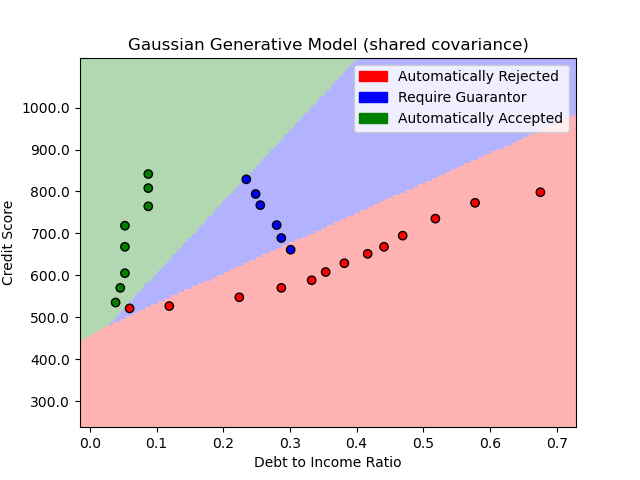
\includegraphics[width=0.45\textwidth]{img_output/Gaussian_Generative_Model_(shared_covariance).png}
    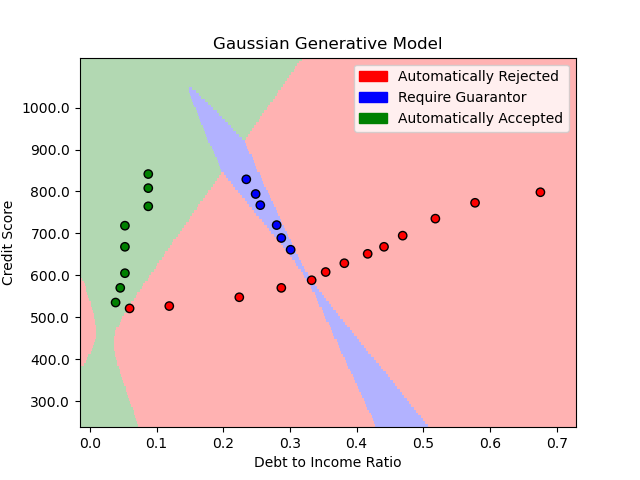
\includegraphics[width=0.45\textwidth]{img_output/Gaussian_Generative_Model.png}
    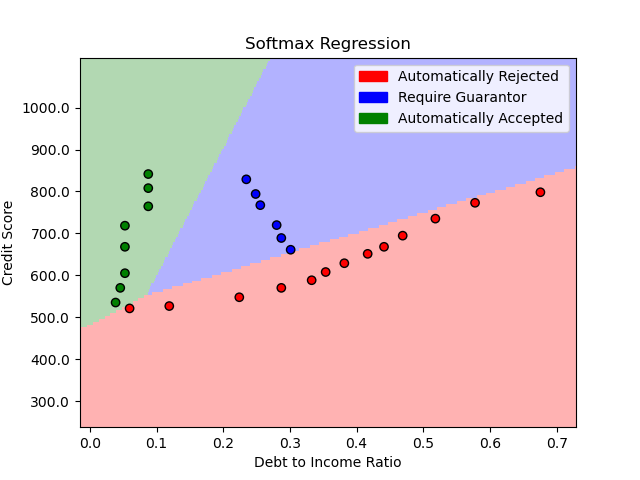
\includegraphics[width=0.45\textwidth]{img_output/softmax.png}
    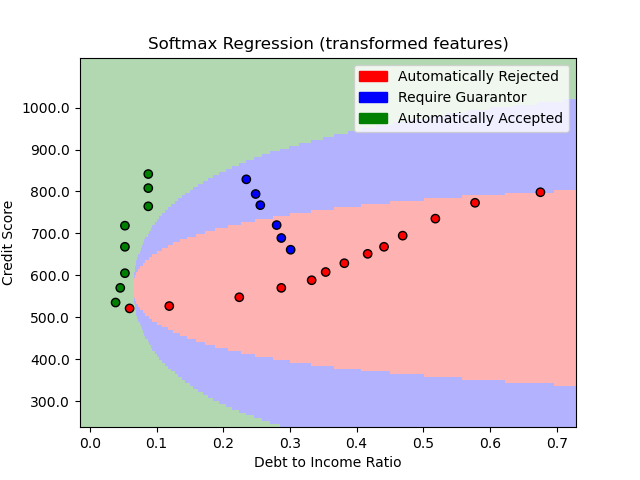
\includegraphics[width=0.45\textwidth]{img_output/softmaxtr.png}
    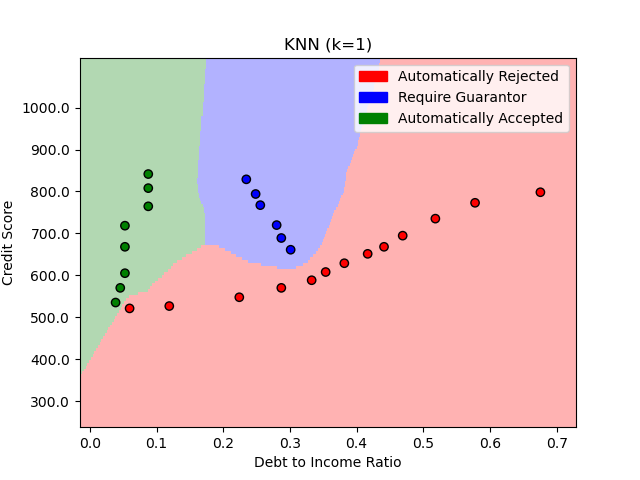
\includegraphics[width=0.45\textwidth]{img_output/KNN1.png}
    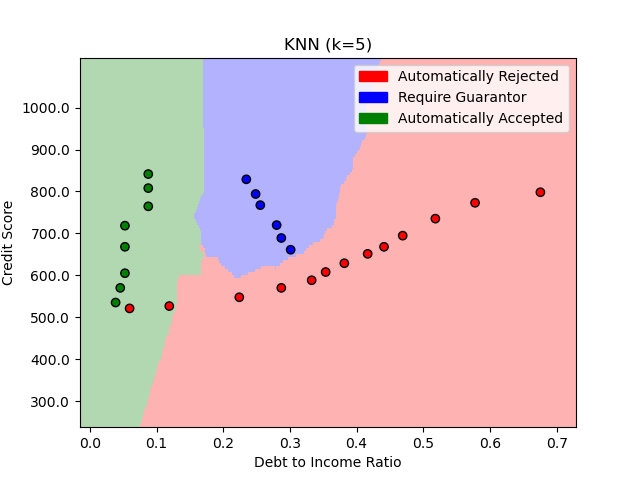
\includegraphics[width=0.45\textwidth]{img_output/KNN5.png}
  \end{center}
  From top to bottom, note that when covariance is shared, our decision boundaries are linear. When covariance is separate for each class, the decision boundaries are quadratic. \par
  The softmax regression without transformed features has linear boundaries, which makes sense because of the setup of softmax. However, our transformation basis is not linear, which results in nonlinear decision boundaries for the transformed features softmax regression. \par
  The kNN classifier with $k=1$ and $k=5$ both have very interesting boundaries, but their shapes are roughly the same. You can see traces of overfitting between the automatically rejected and automatically accepted regions, with every single point in our training data being classified correctly. \par
  \item[2.] Implementation is in the Python Notebook: we have that every model classifies this individual as 0 (rejected) except for softmax regression with transformed features, which classifies the individual as 1 (requires guarantor). \par 
  The probabilities are as follows:
  Softmax regression: $[1.00000000e+00, 9.93305871e-24, 4.05542149e-34]$\par
  Softmax regression with transformed features: $[2.16186498e-01, 7.83763958e-01, 4.95440650e-05]$ \par
  We can see that the softmax regression is very confident, but softmax regression with transformed features is only ~80\% confident. When a piece of data is far from the training data, we are making extrapolations that are not really backed by any confidence. This is especially true for the softmax regression with transformed features, which is not as confident as the other models (since it uses non-linear decision boundaries). \par
  \item[3.] An ethical problem here is that a high debt-to-income ratio is very multi-dimensional. For example, someone who just graduated college might have a lot of debt and a relatively low income, yet they are more trustworthy than someone who might have no debt because they are always getting helped by others, yet also have no income so essentially no way of paying back the loan. A classifier with only two parameters cannot reasonably predict something with as many confounding variables as loan trustworthiness. \par
  In addition to credit score + debt-to-income ratio, we can also consider things like net worth, current career average salary, as well as averages over the past few years to get a better idea of the applicant's current financial situation. 
  \end{itemize}
\end{solution}
\newpage
%%%%%%%%%%%%%%%%%%%%%%%%%%%%%%%%%%%%%%%%%%%%%
% Name and Calibration
%%%%%%%%%%%%%%%%%%%%%%%%%%%%%%%%%%%%%%%%%%%%%
\newpage

\textbf{Name}: Zihongbo Wang

\textbf{Collaborators and Resources}: Ossimi Ziv, Ryan Jiang, and the CS181 Textbook (as well as a youtube video about trolls 2 that clarified naive bayes)

\end{document}
